\documentclass[UTF8]{ctexart}
\usepackage{cite}
\usepackage{graphicx}
\usepackage{subfigure}
\bibliographystyle{IEEEtran}

\begin{document}
	
	\title{关于代码克隆检测的课程报告}
	\author{汤沁予}
	\date{March 11, 2020}
	\maketitle
	
\begin{abstract}
	这篇课程报告主要介绍了代码克隆相关的一些内容。本文首先对代码克隆的定义和影响进行了简要概括,然后介绍了具体应当如何衡量代码相似程度。之后,本文对一些经典的代码克隆检测技术和代码克隆检测质量分析技术进行了简单的介绍。最后对其未来发展趋势进行了一些展望。
	%摘要部分对全文内容做一个大体的介绍,每个段落用大约一句话简单概括。
\end{abstract}

\section{背景}
代码克隆是软件开发中的一种常见行为。\cite{Min2019}中指出,有调查表明,大约5\%到20\%的软件系统中包含克隆代码。

代码克隆通常来源于开发者的复制粘贴行为,或是不同开发者实现相同功能的代码。这固然可以一定程度上减少软件开发的工作量,但同时也会带来许多问题。如下所示:

\begin{enumerate}
	\item 代码克隆会导致源代码的规模增大,即冗余,增加了资源的需求。这对嵌入式系统和手持设备的影响尤为明显。
	\item 克隆一段含有未知bug的代码,可能会导致bug的繁育。
	\item 维护者修改一段代码时,需对这段代码的所有克隆进行一致的修改,若修改不一致则会引入新的bug。
\end{enumerate}

因此,代码克隆被广泛认为是一种代码异味。在开发过程中,通过持续对源代码进行监控管理,以此来检测并去除系统中已有的克隆代码,并防止新克隆的引入,这是很有益处的。

%简要谈一谈什么是代码克隆,会在实际软件的维护和演化中产生什么样的影响,为什么需要进行代码克隆检测。

\section{问题定义}
克隆代码,指的是软件系统中完全相同或是非常相似的两个或多个代码段。而如何衡量两段代码之间的相似性,便是代码克隆检测中较为关键的一个问题。

根据一种较为公认的分类方式,大体上,两段代码之间的相似可以分为两种。一种是基于代码文本的相似,另一种则是基于功能的相似。

\subsection{基于代码文本的相似}

基于代码文本的相似可以分为以下三类:

\begin{description}
	\item[Type I] 只有空白符、代码布局、注释不同,其他地方完全相同。
	\item[Type II] 只有标识符、字面值(literals)、类型、布局和注释不同,在结构、语法上相同。
	\item[Type III] 除了标识符、字面值、类型、布局和注释的不同之外,语句还有可能被修改、增加和删除。
\end{description}

\subsection{基于功能的相似}

而基于功能的相似也被称为语义克隆( semantic clones)。它也被称为Type IV克隆。

\begin{description}
	\item[Type IV] 在语法上不相似,但是仍然在语义上相同。
\end{description}

比如说,分别用冒泡排序和快速排序实现的排序代码块。

\subsection{检测难度}

从Type I到Type IV,克隆的检测难度逐渐上升。

%介绍什么样的代码段对会被认为是克隆代码,代码克隆公认的四个类型以及几种不同的分类方法。

\section{方法和技术}
\label{sec:methods} 
\cite{Min2019}中,根据程序的预处理方法对克隆检测技术大致作了一个分类,分为基于文本、基于标记、基于树、基于程序依赖图以及基于度量这五种。

\subsection{基于文本的克隆检测技术}

基于文本的技术是一类较为朴素的检测技术。除了去除空白行、去除注释等一些最基础的标准化操作外,在两个代码段被比较之前,这类方法几乎不会对源代码进行任何预处理。

在这类克隆检测技术中,源程序代码会被分解为一系列字符串,通常是按行来进行分解。在检测过程中,我们需要找到多个待检测代码中相同的字符串的序列,以此来判断是否为克隆对。

基于文本的克隆检测技术通常只能检测出Type I克隆。

\subsection{基于标记的克隆检测技术}

在基于标记的克隆检测技术中,方法首先要对整个源码系统进行预处理,用词法分析、句法分析等转换方法,将其转换为一个标记(token)的序列。这些序列随后会被检测程序扫描,找出重复的子序列。最终,携带重复子序列的源码段将会被识别为克隆代码段。

与基于文本的方法相比,基于标记的方法对于代码的更改更具有鲁棒性,即使编程者在进行复制粘贴行为后对代码进行了一些代码格式上的改变,也能识别出代码克隆。

基于标记的克隆检测技术除了能检测出Type I克隆外,还能对Type II克隆和部分Type III克隆进行检测。

一个较为典型的、效果达到state of the art的检测方法是CCFinder\cite{Kamiya2002}。图\ref{CCFinder}为该方法论文中附有的流程图。

在该方法中,首先,源代码的每一行都会被用词法分析器转换为若干标记。随后,所有源文件中的多个标记序列会被连接到一起,构成一整个标记序列。这个标记序列将会按照一定的规则进行添加、更改和删除等转换操作。这一步转换操作旨在规范代码中的标识符并识别代码结构。之后,与类型、变量和常量相关的每个标识符将替换为特殊标记。这一步操作使得具有不同变量名的两个代码段能够被识别为克隆代码。接着,方法采取了一种基于后缀树的子字符串匹配算法,来查找转换的标记序列上的类似子序列,其中类似的子序列对返回为克隆对或克隆类。在获得这些标记序列上的克隆对或克隆类信息后,便可以将其映射到源代码上,获得源代码上的克隆对或克隆类。

\begin{figure}[h]
	\centering
	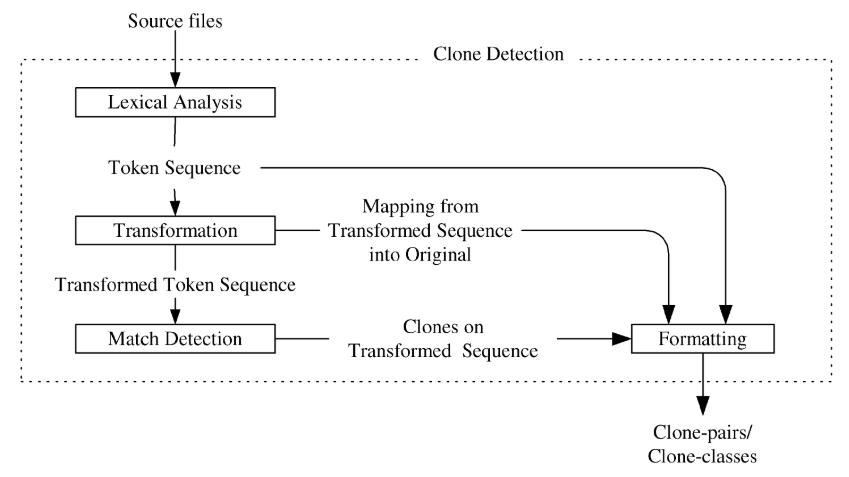
\includegraphics[height=5cm]{Figures/CCFinder}
	\caption{CCFinder论文中附有的流程图}
	\label{CCFinder}
\end{figure}

\subsection{基于树的克隆检测技术}

在基于树的方法中,待检测程序会被用对应语言的语法分析器分解为一棵语法分析树或是抽象语法树。之后,则需要用树匹配算法来在其中搜索相似的子树,这些相似子树对应的源代码便是克隆代码对。

DECKARD\cite{Jiang2007}就是一种基于树的方法。

\subsection{基于程序依赖图的克隆检测技术}

基于程序依赖图的克隆检测又被称为基于语义的克隆检测。程序依赖图包含了代码的控制流和数据流信息,因此我们可以从中得到程序的语义信息。因此,与前面提到的这些方法相比,基于程序依赖图的克隆检测技术能够获取更高层次抽象的代码表示。

在获取了目标代码的程序依赖图后,我们可以使用同构子图检测算法,来寻找整个程序依赖图中相似的子图,从而判断克隆代码对。

\subsection{基于度量的克隆检测技术}

基于度量的克隆检测并不直接对代码进行比较,而是会收集代码段的一些度量来组成向量,对这些向量进行处理和比较。

在这类克隆检测技术中,如何对这些度量进行选择和计算就成为了关键的问题。

%介绍代码克隆检测方法的几个大致的分类,并在每个分类中举例经典的算法进行较为详细的讨论。

\section{代码克隆检测质量分析}
简单介绍判断代码克隆检测方法质量高低的分析方法。

\section{发展趋势}
在第~\ref{sec:methods}章中,提及了几种代码克隆检测技术的分类。除了上述提到的分类外,许多方法并不是纯粹采用其中的某一种,而是将多种预处理技术混合使用,以达到更好的效果。

此外,近年来,随着深度学习在诸多领域取得的广泛成功,许多研究者对深度学习在代码克隆检测上的应用产生了很大的兴趣。

比如,2019年的一篇论文\cite{Yu2019}就使用了基于树和基于度量的混合方法。在该方法中,对于训练数据中的大量代码段,首先被分别生成AST+,然后AST+的每个节点中的单词都会被转化为向量。之后,对处理后的AST+应用基于树的卷积,使用一系列三角形的、深度固定的特征探测器,在树上进行滑动,获取子树的特征。此后,在输出向量的每一个维度上都进行max pooling。这样将任何深度的AST+都转化为一个固定长度的向量。之后,对这些向量两两计算cosin相似度,作为代码段对是否相似的判断。定义损失函数为是否相似的ground truth(0或1)与计算所得cosin相似度之差的平方和,对模型进行训练,最终获得能对任意两段代码判定相似度的网络。这样训练得到的网络能够对最难检测出的Type IV克隆进行检测。


%介绍代码克隆检测目前还存在的一些有待挖掘的研究方向和未来可能的发展趋势。

\bibliography{paper}
\end{document}